\begin{frame}
\frametitle{A Theory of Dynamical Facilitation: Technical Summary}

\begin{enumerate}
    \item<1-> Glassy dynamics via a master equation, governing a hopping process from IS $\alpha$ to another IS $\alpha^\prime$:
    \begin{gather*}
    \frac{\diff p_\alpha(t)}{\diff t} = \sum_{\alpha^\prime} w_{\alpha \alpha^\prime} p_{\alpha^\prime}(t) - w_{\alpha^\prime \alpha}p_\alpha(t) \,, 
    %\begin{equation}
    \quad w_{\alpha^\prime \alpha } = \nu_\mathrm{0} e^{-\beta \Delta F_{\alpha^\prime \alpha}^\ddagger} \,. %\label{eq:transitionrate} \label{eq:mastereq}
    \end{gather*}
    \item<2-> Energy barrier to create a new excitation (labeled $\mu$) is based on elasticity theory:
    %The stress interaction term becomes a pair potential
    %:
    \begin{gather*}
    \Delta F_{\alpha^\prime \alpha}^\ddagger = J_\sigma + \km{\sum_{\mu \prime \neq \mu} v_\mathrm{int}^{\mu  \mu^\prime}} \only<3->{\,, \quad  v^{\mu \mu^\prime}_\mathrm{int} =
    \frac{4\km{\kappa}J_\sigma R_\mathrm{exc}^2}{(r^{\mu \mu^\prime})^2} \cos \left( 2\psi^\mu+2\psi^{\mu^\prime}-4\theta^{\mu \mu^\prime} \right) \,.
    }
    \\
    \only<3->{\km{\kappa \ :} \ \text{interaction strength parameter}}
    \end{gather*}
    \only<3>{
    \centering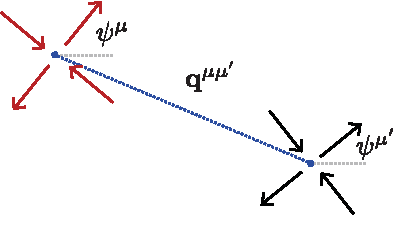
\includegraphics[width=0.5\linewidth]{2.c-fac_intrc/excconfig2.pdf}
    }
    \only<4>{
    \centering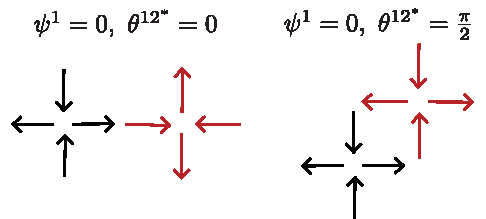
\includegraphics[width=0.6\linewidth]{3.c-fac_results/minima.pdf}
    }
    \item<5-> \textbf{Reversibility:} The energy barrier to create an excitation ($\alpha \to \alpha^\prime$) is the same as reverting the same excitation ($\alpha^\prime \to \alpha$):
    \onslide<6->{
    \begin{equation*}
    \Delta F_{\alpha \alpha^\prime}^\ddagger = \Delta F_{\alpha^\prime \alpha}^\ddagger \only<5->{\  \centering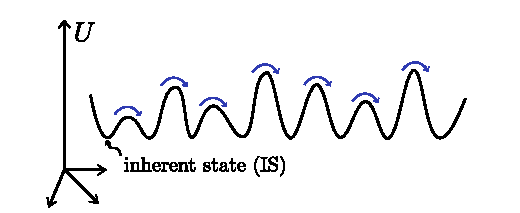
\includegraphics[valign=c,width=0.425\linewidth]{2.c-fac_intrc/pes.pdf}}
    \end{equation*}
    }
    %\begin{figure}
    
    %\end{figure}
    % Given excitation $\mathrm{State} \ 0 \to 1$: Excitation emerges when crossing the first transition state
    % \begin{equation*}
    % \onslide<3->{\Delta F^\ddagger_{10} = J_\sigma}
    % \end{equation*}
    % \item<4-> Excitation leaves behind \textbf{mechanical stress $T_{ij}^1(\* x-\* q^\mu; \psi^\mu)$}
    % \item<5-> $\mathrm{State} \ 1 \to 2$: Second excitation emerges in the presence of previous excitation:
    % \onslide<6->{
    % \begin{equation*}
    % \Delta F^\ddagger_{21} = J_\sigma+\km{\int \diff^2 \* x \ T_{ij}^1 d_{ij}^\ddagger }
    % \end{equation*}
    %}
\end{enumerate}

% \begin{columns}[T]
% \begin{column}[T]{0.5\textwidth}

% \begin{figure}[t]
% %\includegraphics[height=0.65\textheight]{figures/pel_hopping.png}
% \begin{overprint}
% \vspace{12pt}
% \onslide<2>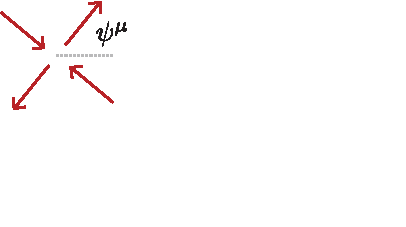
\includegraphics[width=\linewidth]{2.c-fac_intrc/excconfig1.pdf}%\caption{Excitation configuration for the state 1 $\to$ 2 transition.}
% \onslide<3-8>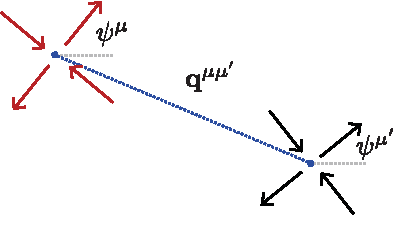
\includegraphics[width=\linewidth]{2.c-fac_intrc/excconfig2.pdf}\only<3-6>{
% \small
% \begin{align*}
% \* q^{\mu \mu^\prime} = \* q^\mu -\* q^{\mu^\prime}: & \ \text{pairwise distance vector}
% \\
% \onslide<4->{q^{\mu \mu^\prime} = \left|\* q^{\mu \mu^\prime}\right|: & \ \text{magnitude of $\* q^{\mu \mu^\prime}$}
% \\
% \theta^{\mu \mu^\prime}: & \ \text{polar angle of $\* q^{\mu\mu^\prime}$}
% \\
% \sigma_\mathrm{exc}: & \ \text{excitation diameter}
% \\
% \km{\kappa}: & \ \text{interaction strength}
% }
% \end{align*}
% }%
% \only<7->{
% \begin{center}
% \begin{block}{\centering Important Note}
% At low temperatures, minima of $v_\mathrm{int}^{\mu \mu^\prime}$ yield most probable excitation \onslide<11->{$\to$ excitation facilitates excitations!}
% \end{block}
% \end{center}
% }

% \onslide<9>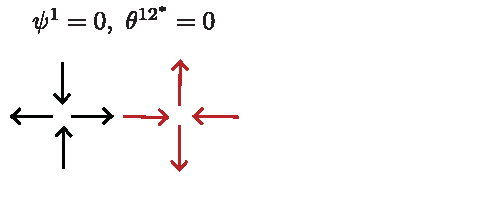
\includegraphics[width=\linewidth]{2.c-fac_intrc/bestprofile1.pdf}
% \begin{center}
% \begin{block}{\centering Important Note}
% At low temperatures, minima of $v_\mathrm{int}^{\mu \mu^\prime}$ yield most probable excitation \onslide<11->{$\to$ excitation facilitates excitations!}
% \end{block}
% \end{center}

% \onslide<10->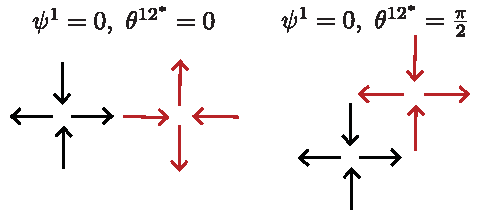
\includegraphics[width=\linewidth]{2.c-fac_intrc/bestprofile.pdf}
% \begin{center}
% \begin{block}{\centering Important Note}
% At low temperatures, minima of $v_\mathrm{int}^{\mu \mu^\prime}$ yield most probable excitation \onslide<11->{$\to$ excitation facilitates excitations!}
% \end{block}
% \end{center}

% \end{overprint}
% \end{figure}


% \end{column}

% \begin{column}[T]{0.5\textwidth}

% \end{column}
% \end{columns}

\end{frame}
% \begin{frame}
% \frametitle{A Theory of Dynamical Facilitation: Summary}

% \begin{columns}[T]
% \begin{column}[T]{0.5\textwidth}

% \begin{figure}[t]
% %\includegraphics[height=0.65\textheight]{figures/pel_hopping.png}
% \begin{overprint}
% \vspace{12pt}
% \onslide<2>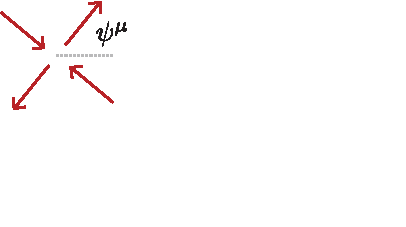
\includegraphics[width=\linewidth]{2.c-fac_intrc/excconfig1.pdf}%\caption{Excitation configuration for the state 1 $\to$ 2 transition.}
% \onslide<3-8>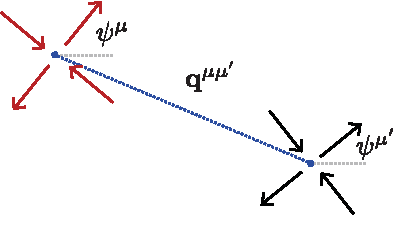
\includegraphics[width=\linewidth]{2.c-fac_intrc/excconfig2.pdf}\only<3-6>{
% \small
% \begin{align*}
% \* q^{\mu \mu^\prime} = \* q^\mu -\* q^{\mu^\prime}: & \ \text{pairwise distance vector}
% \\
% \onslide<4->{q^{\mu \mu^\prime} = \left|\* q^{\mu \mu^\prime}\right|: & \ \text{magnitude of $\* q^{\mu \mu^\prime}$}
% \\
% \theta^{\mu \mu^\prime}: & \ \text{polar angle of $\* q^{\mu\mu^\prime}$}
% \\
% \sigma_\mathrm{exc}: & \ \text{excitation diameter}
% \\
% \km{\kappa}: & \ \text{interaction strength}
% }
% \end{align*}
% }%
% \only<7->{
% \begin{center}
% \begin{block}{\centering Important Note}
% At low temperatures, minima of $v_\mathrm{int}^{\mu \mu^\prime}$ yield most probable excitation \onslide<11->{$\to$ excitation facilitates excitations!}
% \end{block}
% \end{center}
% }

% \onslide<9>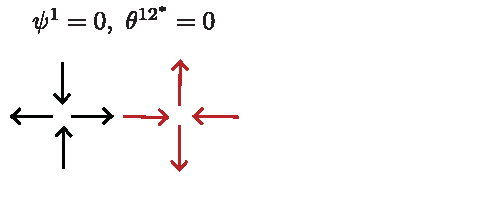
\includegraphics[width=\linewidth]{2.c-fac_intrc/bestprofile1.pdf}
% \begin{center}
% \begin{block}{\centering Important Note}
% At low temperatures, minima of $v_\mathrm{int}^{\mu \mu^\prime}$ yield most probable excitation \onslide<11->{$\to$ excitation facilitates excitations!}
% \end{block}
% \end{center}

% \onslide<10->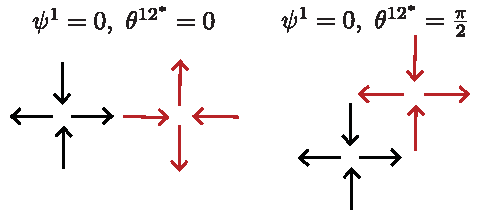
\includegraphics[width=\linewidth]{2.c-fac_intrc/bestprofile.pdf}
% \begin{center}
% \begin{block}{\centering Important Note}
% At low temperatures, minima of $v_\mathrm{int}^{\mu \mu^\prime}$ yield most probable excitation \onslide<11->{$\to$ excitation facilitates excitations!}
% \end{block}
% \end{center}

% \end{overprint}
% \end{figure}


% \end{column}

% \begin{column}[T]{0.5\textwidth}

% \begin{itemize}
%     \item<1-> Glassy dynamics as a Markov process, hopping from IS $\alpha$ to another IS $\alpha^\prime$:
    
%     \onslide<2->{(1) Excitation with orientation $\psi^\mu$ and position $\* q^\mu$}\onslide<3->{, and (2) excitation $\psi^{\mu^\prime}$ and position $\* q^{\mu^\prime}$.}
%     \item<4-> The stress interaction term becomes a pair potential%:
%     \onslide<5->{\begin{equation*}
%     v^{\mu \mu^\prime}_\mathrm{int} =
%     \frac{\km{\kappa}J_\sigma \sigma_\mathrm{exc}^2}{(q^{\mu \mu^\prime})^2} \cos \left( 2\psi^\mu+2\psi^{\mu^\prime}-4\theta^{\mu \mu^\prime} \right) %\label{eq:intterm}
%     \end{equation*}
%     }
%     \item<6->  $\mathrm{State} \ 1 \to 2$: $\Delta F_{12}^\ddagger = J_\sigma+v^{21}_\mathrm{int}$
%     %for $\tilde{q}^{\mu \mu^\prime}:= \frac{q^{\mu \mu^\prime}}{\sigma_\mathrm{exc}} \geq 1$ and $v^{\mu \mu^\prime}_\mathrm{int} = \infty$ otherwise.
%     \item<8-> Minimizing $v^{21}_\mathrm{int}$ yields
%     \begin{equation*}
%     \psi^{2*} = 2\theta^{21*}+\pi \left(n+\frac{1}{2}\right) -\psi^1, \ \ \tilde{q}^{21*} = 1  %\label{eq:fminima12}
%     \end{equation*}
%     where $n$ is an integer.
    
%     % Given excitation $\mathrm{State} \ 0 \to 1$: Excitation emerges when crossing the first transition state
%     % \begin{equation*}
%     % \onslide<3->{\Delta F^\ddagger_{10} = J_\sigma}
%     % \end{equation*}
%     % \item<4-> Excitation leaves behind \textbf{mechanical stress $T_{ij}^1(\* x-\* q^\mu; \psi^\mu)$}
%     % \item<5-> $\mathrm{State} \ 1 \to 2$: Second excitation emerges in the presence of previous excitation:
%     % \onslide<6->{
%     % \begin{equation*}
%     % \Delta F^\ddagger_{21} = J_\sigma+\km{\int \diff^2 \* x \ T_{ij}^1 d_{ij}^\ddagger }
%     % \end{equation*}
%     %}
% \end{itemize}

% \end{column}
% \end{columns}

% \end{frame}
